\documentclass[a5j,openany,papersize,oneside]{tbook}
\usepackage{floatflt}
\usepackage{graphicx}
\usepackage{makeidx}

\renewcommand{\prechaptername}{}  %「第」を消す
\renewcommand{\postchaptername}{} %「章」を消す

\renewcommand{\thechapter}{}
\renewcommand{\thesection}{}
\renewcommand{\thesubsection}{}

\makeindex

\begin{document}

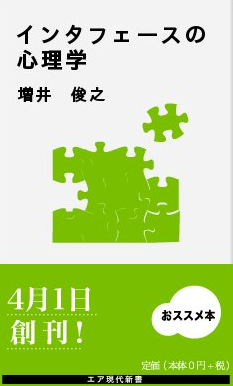
\includegraphics[width=10cm,angle=90,bb=0 0 233 386]{0ace712fba59ecc60fc38d1c93633f6d.png}

\frontmatter
\tableofcontents

\mainmatter

\chapter{インタフェースの心理学}

\section{情報視覚化}

\index{情報視覚化}

\begin{floatingfigure}[r]{60mm}
  \begin{minipage}<y>{9cm}
    \flushright
    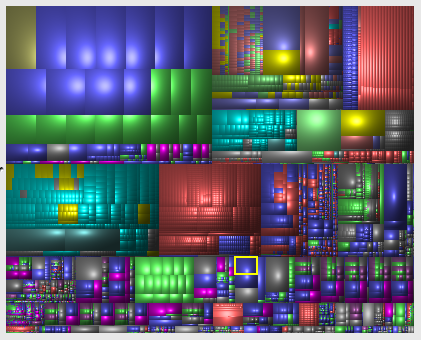
\includegraphics[width=5cm,bb=0 0 421 340]{b8023bc4426a31f2b45e07708d93378e.png}
    \par
    図のサンプル \hfill
  \end{minipage}
\end{floatingfigure}

図\ref{DiskInventoryX}はMacのDisk Inventory Xというソフトで
私のホームディレクトリの中のファイルの大きさを視覚化したものです。
大きなファイルが大きな矩形で表現され、ファイルをまとめたフォルダも矩形として階層的に表現されています。
また下図はWindowsのSequoiaViewというソフトを使ってファイルの大きさを視覚化した例です。
後発のDisk Inventory XはおそらくSequoiaViewに触発されたと思われるので外見がよく似ていますが、
階層的に配置した矩形の集合でファイルサイズを表現するという方法は
University of MarylandのHuman-Computer Interaction Lab\footnote{
  \textsf{http:aaabbbbcc.ccc}
}で開発されたTreeMapというシステムがオリジナルです。



ディスクの中にどんな大きさのファイルがどれほどあるのかはわかりにくいものですが、
TreeMapのような方法を使うと大きなファイルの分布を直感的に把握することができます。
このように、大量の情報をうまく画面上に表示することによって
理解を助けるテクニックを情報視覚化 (\textbf{Information Visualization})と呼びます。

%%%%%%%%%%%%%%%%%

\section{なんとなく、フラクタル}

左の写真の「ロマネスコ」というカリフラワーのように、全体と一部分がどこ
でも同じような形をしているものをフラクタル構造といいます。フラクタル構
造は様々な面白い性質を持っており、比較的簡単に美しいCGを生成するといっ
た応用も多いので、一時かなり話題になりました。

単純なフラクタル構造として、下図のように直線を三分割して折り曲げること
を無限に繰り返してできる コッホ曲線というものが知られています。 縮尺を
大きくするたびに折り曲げを行なうことにすると、 縮尺を3倍にすると長さは
4倍、 縮尺を9倍にすると長さは16倍... という具合に縮尺と長さは変化します
が、 長さと縮尺の対数をとると、その比は常にlog(4)/log(3)=1.2618という一
定の値になり、 この値はフラクタル次元と呼ばれます。

両対数グラフ上にプロットしたグラフが直線になるような関係があるとき、 これらはべき乗則(冪乗則/Power Low)に従うといいます。 フラクタル構造をもつ図形のパラメタはべき乗則に従いますが、 一見フラクタル構造と関係無いところでもべき乗則が成立することがよくあります。 たとえば、文章中でk番目に多く出現する単語の出現頻度は1/kに比例するという Zipf の法則 と呼ばれる経験則がありますが、 この関係は左上図のようにべき乗則に従います。また、富豪の収入もべき乗則に従うと言われています。 世界の長者番付データを もとにしてグラフを書くと下図のようになり、 確かにべき乗則が成立していることがわかります。また最近は インターネットやSNSの様々なパラメタがべき乗則に従うことが発見されており、 これらのフラクタル的な「スケールフリー」構造に関する研究が 注目されています。 べき乗則が観測される場合に必ず厳密なフラクタル構造が存在するとは限りませんが、 何らかのフラクタル的な性質が存在するということは可能です。

\subsection{ご近所のべき分布}

世の中の多くのものは 釣鐘状の正規分布 に従うと一般に信じられている気がしますが、 実際は正規分布をとる現象は世の中では小数派です。 単語の出現頻度も富豪の収入も正規分布にならず、 べき乗則に従うべき分布に従うわけですが、 このような分布は実は全く珍しいものではなく、あらゆる場所で観測することができます。

下の図は、私のホームディレクトリに入っているファイルを 大きさでソートして両対数グラフ上にプロットしたものですが、 単語の出現頻度と同じように、かなり奇麗なべき分布になっていることがわかります。
また下図は、私がメモに使っているWikiサイトのページアクセス回数を 回数でソートして並べたものですが、 やはり奇麗なべき分布になっています。

私のWikiページではアクセス時刻もすべて記憶しているのですが、 アクセスの時間間隔をプロットすると下図のようになり、 やはりべき分布に従っていることがわかります。
このように、私の個人的なファイルについて調べてみると、 あらゆるパラメタがべき分布していることが判明してしまいました。
私は大きなテキストファイルも小さなテキストファイルも持っていますし、 大きな画像ファイルも小さな画像ファイルも持っています。 私の計算機にはこれらの雑多なファイルがまとめて入っているという点が フラクタル的性質の元になっているのでしょう。
メーリングリストのトラフィック、交通渋滞、ネットワークトラフィックなど、 様々な複雑な事象においてべき分布が報告されており、 その発生する理由について様々な解析が行なわれていますが、 どうやら、強い制約が存在しない場合、ほとんどあらゆる状況において 複雑/大規模な事象はべき分布に従うと断言してしまって大丈夫な気がします。 80:20の法則として有名な パレートの法則や、 最近流行の ロングテール現象も すべてべき分布にもとづく性質の表現であり、 このような性質はあたりまえのものなのかもしれません。 ネットワークのような複雑なシステムにおいてはフラクタル的なべき分布が出現するのは当然であり、 その現象が最近発見されて注目されたという点の方が不思議な気がします。
(ベンフォードの法則も?)
■ フラクタル性の応用
複雑なシステムにおいてべき乗則が出現する理由を説明するための 様々なモデルが提案されています。 しかし、あるモデルによって計算した結果が実際と一致していたとしても、 全く異なる方法でも同じような結果が得られる可能性も高いので、 本当にそのモデルが成立しているのかを証明することは難しそうです。 一方、 べき乗則の出現理由についてはわからなくても、 べき乗則を効果的に利用する方法を工夫することは可能です。 世の中のものはほとんどがフラクタル的であることを理解したうえで、 それを考慮したシステムを設計して利用することを考えるとよさそうです。




\backmatter

%\begin{theindex}
% \documentclass[a5j,openany,papersize,oneside]{tbook}
\usepackage{floatflt}
\usepackage{graphicx}
\usepackage{makeidx}

\renewcommand{\prechaptername}{}  %「第」を消す
\renewcommand{\postchaptername}{} %「章」を消す

\renewcommand{\thechapter}{}
\renewcommand{\thesection}{}
\renewcommand{\thesubsection}{}

\makeindex

\begin{document}

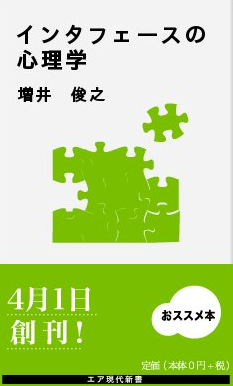
\includegraphics[width=10cm,angle=90,bb=0 0 233 386]{0ace712fba59ecc60fc38d1c93633f6d.png}

\frontmatter
\tableofcontents

\mainmatter

\chapter{インタフェースの心理学}

\section{情報視覚化}

\index{情報視覚化}

\begin{floatingfigure}[r]{60mm}
  \begin{minipage}<y>{9cm}
    \flushright
    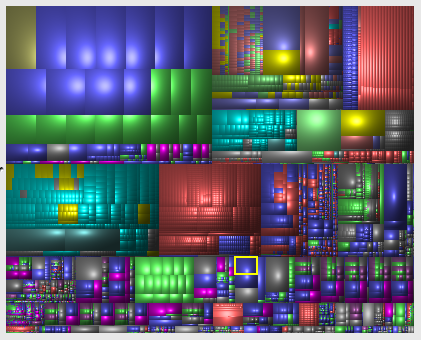
\includegraphics[width=5cm,bb=0 0 421 340]{b8023bc4426a31f2b45e07708d93378e.png}
    \par
    図のサンプル \hfill
  \end{minipage}
\end{floatingfigure}

図\ref{DiskInventoryX}はMacのDisk Inventory Xというソフトで
私のホームディレクトリの中のファイルの大きさを視覚化したものです。
大きなファイルが大きな矩形で表現され、ファイルをまとめたフォルダも矩形として階層的に表現されています。
また下図はWindowsのSequoiaViewというソフトを使ってファイルの大きさを視覚化した例です。
後発のDisk Inventory XはおそらくSequoiaViewに触発されたと思われるので外見がよく似ていますが、
階層的に配置した矩形の集合でファイルサイズを表現するという方法は
University of MarylandのHuman-Computer Interaction Lab\footnote{
  \textsf{http:aaabbbbcc.ccc}
}で開発されたTreeMapというシステムがオリジナルです。



ディスクの中にどんな大きさのファイルがどれほどあるのかはわかりにくいものですが、
TreeMapのような方法を使うと大きなファイルの分布を直感的に把握することができます。
このように、大量の情報をうまく画面上に表示することによって
理解を助けるテクニックを情報視覚化 (\textbf{Information Visualization})と呼びます。

%%%%%%%%%%%%%%%%%

\section{なんとなく、フラクタル}

左の写真の「ロマネスコ」というカリフラワーのように、全体と一部分がどこ
でも同じような形をしているものをフラクタル構造といいます。フラクタル構
造は様々な面白い性質を持っており、比較的簡単に美しいCGを生成するといっ
た応用も多いので、一時かなり話題になりました。

単純なフラクタル構造として、下図のように直線を三分割して折り曲げること
を無限に繰り返してできる コッホ曲線というものが知られています。 縮尺を
大きくするたびに折り曲げを行なうことにすると、 縮尺を3倍にすると長さは
4倍、 縮尺を9倍にすると長さは16倍... という具合に縮尺と長さは変化します
が、 長さと縮尺の対数をとると、その比は常にlog(4)/log(3)=1.2618という一
定の値になり、 この値はフラクタル次元と呼ばれます。

両対数グラフ上にプロットしたグラフが直線になるような関係があるとき、 これらはべき乗則(冪乗則/Power Low)に従うといいます。 フラクタル構造をもつ図形のパラメタはべき乗則に従いますが、 一見フラクタル構造と関係無いところでもべき乗則が成立することがよくあります。 たとえば、文章中でk番目に多く出現する単語の出現頻度は1/kに比例するという Zipf の法則 と呼ばれる経験則がありますが、 この関係は左上図のようにべき乗則に従います。また、富豪の収入もべき乗則に従うと言われています。 世界の長者番付データを もとにしてグラフを書くと下図のようになり、 確かにべき乗則が成立していることがわかります。また最近は インターネットやSNSの様々なパラメタがべき乗則に従うことが発見されており、 これらのフラクタル的な「スケールフリー」構造に関する研究が 注目されています。 べき乗則が観測される場合に必ず厳密なフラクタル構造が存在するとは限りませんが、 何らかのフラクタル的な性質が存在するということは可能です。

\subsection{ご近所のべき分布}

世の中の多くのものは 釣鐘状の正規分布 に従うと一般に信じられている気がしますが、 実際は正規分布をとる現象は世の中では小数派です。 単語の出現頻度も富豪の収入も正規分布にならず、 べき乗則に従うべき分布に従うわけですが、 このような分布は実は全く珍しいものではなく、あらゆる場所で観測することができます。

下の図は、私のホームディレクトリに入っているファイルを 大きさでソートして両対数グラフ上にプロットしたものですが、 単語の出現頻度と同じように、かなり奇麗なべき分布になっていることがわかります。
また下図は、私がメモに使っているWikiサイトのページアクセス回数を 回数でソートして並べたものですが、 やはり奇麗なべき分布になっています。

私のWikiページではアクセス時刻もすべて記憶しているのですが、 アクセスの時間間隔をプロットすると下図のようになり、 やはりべき分布に従っていることがわかります。
このように、私の個人的なファイルについて調べてみると、 あらゆるパラメタがべき分布していることが判明してしまいました。
私は大きなテキストファイルも小さなテキストファイルも持っていますし、 大きな画像ファイルも小さな画像ファイルも持っています。 私の計算機にはこれらの雑多なファイルがまとめて入っているという点が フラクタル的性質の元になっているのでしょう。
メーリングリストのトラフィック、交通渋滞、ネットワークトラフィックなど、 様々な複雑な事象においてべき分布が報告されており、 その発生する理由について様々な解析が行なわれていますが、 どうやら、強い制約が存在しない場合、ほとんどあらゆる状況において 複雑/大規模な事象はべき分布に従うと断言してしまって大丈夫な気がします。 80:20の法則として有名な パレートの法則や、 最近流行の ロングテール現象も すべてべき分布にもとづく性質の表現であり、 このような性質はあたりまえのものなのかもしれません。 ネットワークのような複雑なシステムにおいてはフラクタル的なべき分布が出現するのは当然であり、 その現象が最近発見されて注目されたという点の方が不思議な気がします。
(ベンフォードの法則も?)
■ フラクタル性の応用
複雑なシステムにおいてべき乗則が出現する理由を説明するための 様々なモデルが提案されています。 しかし、あるモデルによって計算した結果が実際と一致していたとしても、 全く異なる方法でも同じような結果が得られる可能性も高いので、 本当にそのモデルが成立しているのかを証明することは難しそうです。 一方、 べき乗則の出現理由についてはわからなくても、 べき乗則を効果的に利用する方法を工夫することは可能です。 世の中のものはほとんどがフラクタル的であることを理解したうえで、 それを考慮したシステムを設計して利用することを考えるとよさそうです。




\backmatter

%\begin{theindex}
% \documentclass[a5j,openany,papersize,oneside]{tbook}
\usepackage{floatflt}
\usepackage{graphicx}
\usepackage{makeidx}

\renewcommand{\prechaptername}{}  %「第」を消す
\renewcommand{\postchaptername}{} %「章」を消す

\renewcommand{\thechapter}{}
\renewcommand{\thesection}{}
\renewcommand{\thesubsection}{}

\makeindex

\begin{document}

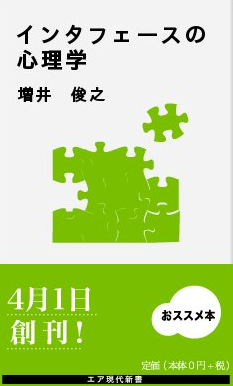
\includegraphics[width=10cm,angle=90,bb=0 0 233 386]{0ace712fba59ecc60fc38d1c93633f6d.png}

\frontmatter
\tableofcontents

\mainmatter

\chapter{インタフェースの心理学}

\section{情報視覚化}

\index{情報視覚化}

\begin{floatingfigure}[r]{60mm}
  \begin{minipage}<y>{9cm}
    \flushright
    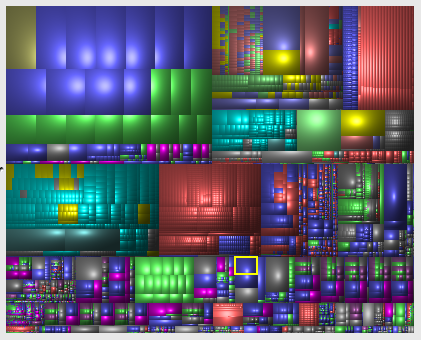
\includegraphics[width=5cm,bb=0 0 421 340]{b8023bc4426a31f2b45e07708d93378e.png}
    \par
    図のサンプル \hfill
  \end{minipage}
\end{floatingfigure}

図\ref{DiskInventoryX}はMacのDisk Inventory Xというソフトで
私のホームディレクトリの中のファイルの大きさを視覚化したものです。
大きなファイルが大きな矩形で表現され、ファイルをまとめたフォルダも矩形として階層的に表現されています。
また下図はWindowsのSequoiaViewというソフトを使ってファイルの大きさを視覚化した例です。
後発のDisk Inventory XはおそらくSequoiaViewに触発されたと思われるので外見がよく似ていますが、
階層的に配置した矩形の集合でファイルサイズを表現するという方法は
University of MarylandのHuman-Computer Interaction Lab\footnote{
  \textsf{http:aaabbbbcc.ccc}
}で開発されたTreeMapというシステムがオリジナルです。



ディスクの中にどんな大きさのファイルがどれほどあるのかはわかりにくいものですが、
TreeMapのような方法を使うと大きなファイルの分布を直感的に把握することができます。
このように、大量の情報をうまく画面上に表示することによって
理解を助けるテクニックを情報視覚化 (\textbf{Information Visualization})と呼びます。

%%%%%%%%%%%%%%%%%

\section{なんとなく、フラクタル}

左の写真の「ロマネスコ」というカリフラワーのように、全体と一部分がどこ
でも同じような形をしているものをフラクタル構造といいます。フラクタル構
造は様々な面白い性質を持っており、比較的簡単に美しいCGを生成するといっ
た応用も多いので、一時かなり話題になりました。

単純なフラクタル構造として、下図のように直線を三分割して折り曲げること
を無限に繰り返してできる コッホ曲線というものが知られています。 縮尺を
大きくするたびに折り曲げを行なうことにすると、 縮尺を3倍にすると長さは
4倍、 縮尺を9倍にすると長さは16倍... という具合に縮尺と長さは変化します
が、 長さと縮尺の対数をとると、その比は常にlog(4)/log(3)=1.2618という一
定の値になり、 この値はフラクタル次元と呼ばれます。

両対数グラフ上にプロットしたグラフが直線になるような関係があるとき、 これらはべき乗則(冪乗則/Power Low)に従うといいます。 フラクタル構造をもつ図形のパラメタはべき乗則に従いますが、 一見フラクタル構造と関係無いところでもべき乗則が成立することがよくあります。 たとえば、文章中でk番目に多く出現する単語の出現頻度は1/kに比例するという Zipf の法則 と呼ばれる経験則がありますが、 この関係は左上図のようにべき乗則に従います。また、富豪の収入もべき乗則に従うと言われています。 世界の長者番付データを もとにしてグラフを書くと下図のようになり、 確かにべき乗則が成立していることがわかります。また最近は インターネットやSNSの様々なパラメタがべき乗則に従うことが発見されており、 これらのフラクタル的な「スケールフリー」構造に関する研究が 注目されています。 べき乗則が観測される場合に必ず厳密なフラクタル構造が存在するとは限りませんが、 何らかのフラクタル的な性質が存在するということは可能です。

\subsection{ご近所のべき分布}

世の中の多くのものは 釣鐘状の正規分布 に従うと一般に信じられている気がしますが、 実際は正規分布をとる現象は世の中では小数派です。 単語の出現頻度も富豪の収入も正規分布にならず、 べき乗則に従うべき分布に従うわけですが、 このような分布は実は全く珍しいものではなく、あらゆる場所で観測することができます。

下の図は、私のホームディレクトリに入っているファイルを 大きさでソートして両対数グラフ上にプロットしたものですが、 単語の出現頻度と同じように、かなり奇麗なべき分布になっていることがわかります。
また下図は、私がメモに使っているWikiサイトのページアクセス回数を 回数でソートして並べたものですが、 やはり奇麗なべき分布になっています。

私のWikiページではアクセス時刻もすべて記憶しているのですが、 アクセスの時間間隔をプロットすると下図のようになり、 やはりべき分布に従っていることがわかります。
このように、私の個人的なファイルについて調べてみると、 あらゆるパラメタがべき分布していることが判明してしまいました。
私は大きなテキストファイルも小さなテキストファイルも持っていますし、 大きな画像ファイルも小さな画像ファイルも持っています。 私の計算機にはこれらの雑多なファイルがまとめて入っているという点が フラクタル的性質の元になっているのでしょう。
メーリングリストのトラフィック、交通渋滞、ネットワークトラフィックなど、 様々な複雑な事象においてべき分布が報告されており、 その発生する理由について様々な解析が行なわれていますが、 どうやら、強い制約が存在しない場合、ほとんどあらゆる状況において 複雑/大規模な事象はべき分布に従うと断言してしまって大丈夫な気がします。 80:20の法則として有名な パレートの法則や、 最近流行の ロングテール現象も すべてべき分布にもとづく性質の表現であり、 このような性質はあたりまえのものなのかもしれません。 ネットワークのような複雑なシステムにおいてはフラクタル的なべき分布が出現するのは当然であり、 その現象が最近発見されて注目されたという点の方が不思議な気がします。
(ベンフォードの法則も?)
■ フラクタル性の応用
複雑なシステムにおいてべき乗則が出現する理由を説明するための 様々なモデルが提案されています。 しかし、あるモデルによって計算した結果が実際と一致していたとしても、 全く異なる方法でも同じような結果が得られる可能性も高いので、 本当にそのモデルが成立しているのかを証明することは難しそうです。 一方、 べき乗則の出現理由についてはわからなくても、 べき乗則を効果的に利用する方法を工夫することは可能です。 世の中のものはほとんどがフラクタル的であることを理解したうえで、 それを考慮したシステムを設計して利用することを考えるとよさそうです。




\backmatter

%\begin{theindex}
% \documentclass[a5j,openany,papersize,oneside]{tbook}
\usepackage{floatflt}
\usepackage{graphicx}
\usepackage{makeidx}

\renewcommand{\prechaptername}{}  %「第」を消す
\renewcommand{\postchaptername}{} %「章」を消す

\renewcommand{\thechapter}{}
\renewcommand{\thesection}{}
\renewcommand{\thesubsection}{}

\makeindex

\begin{document}

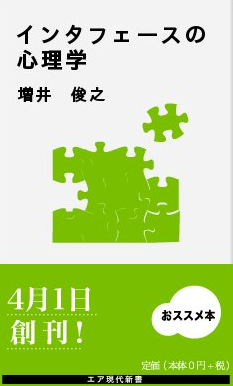
\includegraphics[width=10cm,angle=90,bb=0 0 233 386]{0ace712fba59ecc60fc38d1c93633f6d.png}

\frontmatter
\tableofcontents

\mainmatter

\chapter{インタフェースの心理学}

\section{情報視覚化}

\index{情報視覚化}

\begin{floatingfigure}[r]{60mm}
  \begin{minipage}<y>{9cm}
    \flushright
    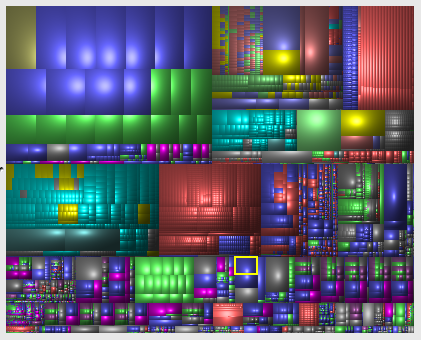
\includegraphics[width=5cm,bb=0 0 421 340]{b8023bc4426a31f2b45e07708d93378e.png}
    \par
    図のサンプル \hfill
  \end{minipage}
\end{floatingfigure}

図\ref{DiskInventoryX}はMacのDisk Inventory Xというソフトで
私のホームディレクトリの中のファイルの大きさを視覚化したものです。
大きなファイルが大きな矩形で表現され、ファイルをまとめたフォルダも矩形として階層的に表現されています。
また下図はWindowsのSequoiaViewというソフトを使ってファイルの大きさを視覚化した例です。
後発のDisk Inventory XはおそらくSequoiaViewに触発されたと思われるので外見がよく似ていますが、
階層的に配置した矩形の集合でファイルサイズを表現するという方法は
University of MarylandのHuman-Computer Interaction Lab\footnote{
  \textsf{http:aaabbbbcc.ccc}
}で開発されたTreeMapというシステムがオリジナルです。



ディスクの中にどんな大きさのファイルがどれほどあるのかはわかりにくいものですが、
TreeMapのような方法を使うと大きなファイルの分布を直感的に把握することができます。
このように、大量の情報をうまく画面上に表示することによって
理解を助けるテクニックを情報視覚化 (\textbf{Information Visualization})と呼びます。

%%%%%%%%%%%%%%%%%

\include{fractal}

\backmatter

%\begin{theindex}
% \include{junk.idx}
\printindex
%\end{theindex}

\end{document}



\printindex
%\end{theindex}

\end{document}



\printindex
%\end{theindex}

\end{document}



\printindex
%\end{theindex}

\end{document}


